\documentclass{beamer}

\usepackage{listings}
\usepackage{graphicx}
\usepackage{stmaryrd}
\usepackage{../assets/style}

\title{Implementation of a Type-Safe Structure Editor}
\author{Tórur, Thorbjørn \& Nicolaj}
\institute{University of Copenhagen}
\date{\today}

\begin{document}

% References
\newcommand\pepm{\cite{10.1145/3441296.3441393}}
\newcommand\cornell{\cite{10.1145/358746.358755}}
\newcommand\hazel{\cite{conf/popl/Hazelnut17}}
\newcommand\scratch{\cite{10.1145/1592761.1592779}}
\newcommand\alice{\cite{10.1145/332040.332481}}
\newcommand\elmcore{\cite{Elm-lang-core}}
\newcommand\elmsvg{\cite{Elm-lang-svg}}
\newcommand\elmmat{\cite{Elm-lang-material}}
\newcommand\elmhtml{\cite{Elm-lang-html}}

% Metadata
\newcommand\mdtitle{Implementation of a Type-Safe Structure Editor}
\newcommand\mdtitleshort{Implementation of a Type-Safe Structure Editor}
\newcommand\mdauthor{
  Nicolaj Richs-Jensen \\
  \url{vzq239@alumni.ku.dk}
  \and
  Thorbjørn Bülow Bringgaard \\
  \url{vwc415@alumni.ku.dk}
  \and
  Tórur Feilberg Zachariasen \\
  \url{xsz482@alumni.ku.dk}
}
\newcommand\mdauthorshort{Nicolaj, Thorbjørn, Tórur \& Hans}
\newcommand\mddate{\today}

% Syntax
\newcommand\app[2]{#1~#2}
\newcommand\abs[2]{\lambda #1.#2}
\newcommand\cursor[1]{\llbracket #1 \rrbracket}
\newcommand\breakpoint[1]{\langle #1 \rangle}
\newcommand\hole{\llparenthesis\rrparenthesis}
\newcommand\transition[1]{\xrightarrow[]{\text{#1}}}

\newcommand\AST{\textbf{Ast}}
\newcommand\Ast{%
  a &::= x
  \mid c
  \mid \app{a_1}{a_2}
  \mid \abs{x}{a}
  \mid \cursor{a}
  \mid \breakpoint{a}
  \mid \hole
}

% Cursor contexts
\newcommand{\cursorhole}{\[\cdot\]}
\newcommand{\Cts}{C &::= [\cdot] \mid \app{C}{\hat{a}} \mid \app{\hat{a}}{C} \mid \abs{x}{C} \mid \breakpoint{C}}

\newcommand\aHat{%
  \hat{a} &::= x
  \mid c
  \mid \app{\hat{a}_1}{\hat{a}_2}
  \mid \abs{x}{\hat{a}}
  \mid \breakpoint{\hat{a}}
  \mid \hole
}

\newcommand\aDot{%
  \dot{a} &::= \cursor{\hat{a}}
  \mid \abs{x}{\cursor{\hat{a}}}
  \mid \app{\cursor{\hat{a}_1}}{\hat{a}_2}
  \mid \app{\hat{a}_1}{\cursor{\hat{a}_2}}
  \mid \breakpoint{\cursor{\hat{a}}}
}

% Editor expressions
\newcommand\pre[2]{#1.#2}
\newcommand\bicond[3]{\ensuremath{#1 \Rightarrow #2 \mid #3}}
\newcommand\seqcomp[2]{\ensuremath{#1 \ggg #2}}
\newcommand\rec[2]{\ensuremath{\texttt{rec}~#1.#2}}
\newcommand\call[1]{#1}
\newcommand\nil{\mathbf{0}}
\newcommand\Exp[2]{\breakpoint{#1,\, #2}}

\newcommand\edt{\textbf{Edt}}
\newcommand\Edt{%
  E &::= \pre{\pi}{E}
  \mid \bicond{\phi}{E_1}{E_2}
  \mid \seqcomp{E_1}{E_2}
  \mid \rec{x}{E}
  \mid \call{x}
  \mid \nil
}

% Prefix commands
\newcommand\eval{\texttt{eval}}
\newcommand\sub[1]{\ensuremath{\{ #1 \}}}
\newcommand\child[1]{\ensuremath{\texttt{child}~#1}}
\newcommand\parent{\texttt{parent}}

\newcommand\aep{\textbf{Aep}}
\newcommand\Aep{%
  \pi &::= \eval
  \mid \sub{D}
  \mid \child{n}
  \mid \parent
}

% AST node modifiers
\newcommand\var[1]{\texttt{var}~x}
\newcommand\const[1]{\texttt{const}~c}
\newcommand\aamApp{\texttt{app}}
\newcommand\aamLambda[1]{\texttt{lambda}~#1}
\newcommand\aamBreak{\texttt{break}}
\newcommand\aamHole{\texttt{hole}}

\newcommand\aam{\textbf{Aam}}
\newcommand\Aam{%
  D &::= \var{x}
  \mid \const{c}
  \mid \aamApp
  \mid \aamLambda{x}
  \mid \aamBreak
  \mid \aamHole
}

% Conditions
\newcommand\conjunction[2]{#1 \land #2}
\newcommand\disjunction[2]{#1 \lor #2}
\newcommand\at[1]{@#1}
\newcommand\possibly[1]{\Diamond #1}
\newcommand\necessarily[1]{\Box #1}

\newcommand\eed{\textbf{Eed}}
\newcommand\Eed{%
  \phi &::= \neg\phi
  \mid \conjunction{\phi_1}{\phi_2}
  \mid \disjunction{\phi_1}{\phi_2}
  \mid \at{D}
  \mid \possibly{D}
  \mid \necessarily{D}
}

% Reduction rules
%% Table 1
\newcommand\CondOne{%
  \frac{a \vDash \phi}
  {\Exp{\bicond{\phi}{E_1}{E_2}}{a}\transition{$\epsilon$}\Exp{E_1}{a}}
}

\newcommand\CondTwo{%
  \frac{a \nvDash \phi}
  {\Exp{\bicond{\phi}{E_1}{E_2}}{a}\transition{$\epsilon$}\Exp{E_2}{a}}
}

\newcommand\Eval{%
  \frac{a \to v}
  {\Exp{\pre{\eval}{E}}{a}\transition{$v$}\Exp{E}{a}}
}

\newcommand\Seq{%
  \frac{\Exp{E_1}{a}\transition{$\alpha$}\Exp{E_1'}{a'}}
  {\Exp{\seqcomp{E_1}{E_2}}{a}\transition{$\alpha$}\Exp{\seqcomp{E_1'}{E_2}}{a'}}
}

\newcommand\Struct{%
  \frac{E_1 \equiv E_2\quad\Exp{E_2}{a}\transition{$\alpha$}\Exp{E_2'}{a'} \quad E_2' \equiv E_1'}
  {\Exp{E_1}{a}\transition{$\alpha$}\Exp{E_1'}{a'}}
}

\newcommand\Context{%
  \begin{aligned}
     & \frac{a \transition{$\pi$} a'}
    {\Exp{\pre{\pi}{E}}{C[a]}\transition{$\pi$}\Exp{E}{C[a']}} \\
     & \text{where } \pi \neq \eval
  \end{aligned}
}

%% Table 2
\newcommand\Var{%
  \frac{}
  {\cursor{\hat{a}}\transition{\{var x\}}\cursor{x}}
}

\newcommand\Hole{%
  \frac{}
  {\cursor{\hat{a}}\transition{\{hole\}}\cursor{\hole}}
}

\newcommand\Const{%
  \frac{}
  {\cursor{\hat{a}}\transition{\{const c\}}\cursor{c}}
}

\newcommand\App{%
  \frac{}
  {\cursor{\hat{a}}\transition{\{app\}}\cursor{\app{\hole}{\hole}}}
}

\newcommand\BreakOne{%
  \frac{\hat{a} \neq \breakpoint{\hat{a}'}}
  {\cursor{\hat{a}}\transition{\{break\}}\cursor{\breakpoint{\hat{a}}}}
}

\newcommand\BreakTwo{%
  \frac{}
  {\cursor{\breakpoint{\hat{a}}}\transition{\{break\}}\cursor{\hat{a}}}
}

\newcommand\LAMBDA{%
  \frac{}
  {\cursor{\hat{a}}\transition{\{lambda x\}}\cursor{\abs{x}{\hole}}}
}

%% Table 3
\newcommand\AppCOne{%
  \frac{}
  {\cursor{\app{\hat{a}_1}{\hat{a}_2}}\transition{child 1}\app{\cursor{\hat{a}_1}}{\hat{a}_2}}
}

\newcommand\AppCTwo{%
  \frac{}
  {\cursor{\app{\hat{a}_1}{\hat{a}_2}}\transition{child 2}\app{\hat{a}_1}{\cursor{\hat{a}_2}}}
}

\newcommand\AppPOne{%
  \frac{}
  {\app{\cursor{\hat{a}_1}}{\hat{a}_2}\transition{parent}\cursor{\app{\hat{a}_1}{\hat{a}_2}}}
}

\newcommand\AppPTwo{%
  \frac{}
  {\app{\hat{a}_1}{\cursor{\hat{a}_2}}\transition{parent}\cursor{\app{\hat{a}_1}{\hat{a}_2}}}
}

\newcommand\ABSC{%
  \frac{}
  {\cursor{\abs{x}{\hat{a}}}\transition{child 1}\abs{x}{\cursor{\hat{a}}}}
}

\newcommand\ABSP{%
  \frac{}
  {\abs{x}{\cursor{\hat{a}}}\transition{parent}\cursor{\abs{x}{\hat{a}}}}
}

\newcommand\BreakC{%
  \frac{}
  {\cursor{\breakpoint{\hat{a}}}\transition{child 1}\breakpoint{\cursor{\hat{a}}}}
}

\newcommand\BreakP{%
  \frac{}
  {\breakpoint{\cursor{\hat{a}}}\transition{parent}\cursor{\breakpoint{\hat{a}}}}
}

%% Table 4
\newcommand\AtVar{%
  \frac{}
  {x \vDash \at{(\text{var }y)}}
}

\newcommand\AtConst{%
  \frac{}
  {c \vDash \at{(\text{const }c)}}
}

\newcommand\AtHole{%
  \frac{}
  {\hole \vDash \at{\text{hole}}}
}

\newcommand\AtApp{%
  \frac{}
  {\app{\hat{a}_1}{\hat{a}_2} \vDash \at{\text{app}}}
}

\newcommand\AtAbs{%
  \frac{}
  {\abs{x}{\hat{a}} \vDash \at{\text{lambda }y}}
}

\newcommand\AtBreak{%
  \frac{}
  {\breakpoint{\hat{a}} \vDash \at{\text{break}}}
}

%% Table 5
\newcommand\PosTrivial{%
  \frac{\hat{a} \vDash \at{D}}
  {\hat{a} \vDash \possibly{D}}
}

\newcommand\PosAppOne{%
  \frac{\hat{a}_1 \vDash \possibly{D}}
  {\app{\hat{a}_1}{\hat{a}_2} \vDash \possibly{D}}
}

\newcommand\PosAppTwo{%
  \frac{\hat{a}_2 \vDash \possibly{D}}
  {\app{\hat{a}_1}{\hat{a}_2} \vDash \possibly{D}}
}

\newcommand\PosAbs{%
  \frac{\hat{a} \vDash \possibly{D}}
  {\abs{x}{\hat{a}} \vDash \possibly{D}}
}

\newcommand\PosBreak{%
  \frac{\hat{a} \vDash \possibly{D}}
  {\breakpoint{\hat{a}} \vDash \possibly{D}}
}

\newcommand\NecTrivial{%
  \frac{\hat{a} \vDash \at{D}}
  {\hat{a} \vDash \necessarily{D}}
}

\newcommand\NecApp{%
  \frac{\hat{a}_1 \vDash \possibly{D}\quad\hat{a}_2 \vDash \possibly{D}}
  {\app{\hat{a}_1}{\hat{a}_2} \vDash \necessarily{D}}
}

\newcommand\NecAbs{%
  \frac{\hat{a} \vDash \possibly{D}}
  {\abs{x}{\hat{a}} \vDash \necessarily{D}}
}

\newcommand\NecBreak{%
  \frac{\hat{a} \vDash \possibly{D}}
  {\breakpoint{\hat{a}} \vDash \necessarily{D}}
}


%% Table 6
\newcommand\BConst{%
  \frac{}
  {c \to c}
}

\newcommand\BAbs{%
  \frac{}
  {\abs{x}{a}\to\abs{x}{a}}
}

\newcommand\BCursor{%
  \frac{a \to v}
  {\cursor{a} \to v}
}

\newcommand\BApp{%
  \begin{aligned}
     & \frac{a_1 \to \abs{x}{a_1'} \quad a_2 \to v \quad a_1'\{v/x\} \to v'}
    {\app{a_1}{a_2} \to v'}                                                  \\
     & \text{where } v \notin \textbf{BVal} \cup \textbf{HVal}
  \end{aligned}
}

\newcommand\BAppBOne{%
  \frac{a_1 \to w}
  {\app{a_1}{a_2} \to \app{w}{a_2}}
}

\newcommand\BAppBTwo{%
  \frac{a_1 \to \abs{x}{a_1'} \quad a_2 \to w}
  {\app{a_1}{a_2} \to \app{\abs{x}{a_1'}}{w}}
}

\newcommand\BAppHOne{%
  \frac{a_1 \to u \quad a_2 \to v}
  {\app{a_1}{a_2} \to \app{u}{v}}
}

\newcommand\BAppHTwo{%
  \frac{a_1 \to \abs{x}{a_1'} \quad a_2 \to u}
  {\app{a_1}{a_2} \to \app{\abs{x}{a_1'}}{u}}
}

\newcommand\BBreakB{%
  \frac{}
  {\breakpoint{a}\to\breakpoint{a}}
}


% Values
\newcommand\val{\textbf{Val}}
\newcommand\Val{%
  v &::= c
  \mid \abs{x}{a}
  \mid w
  \mid u
}

\newcommand\hval{\textbf{HVal}}
\newcommand\HVal{%
  u &::= \hole
  \mid \app{u}{v}
  \mid \app{\abs{x}{a}}{u}
}

\newcommand\bval{\textbf{BVal}}
\newcommand\BVal{%
  w &::= \breakpoint{a}
  \mid \app{w}{a}
  \mid \app{\abs{x}{a}}{w}
}


% Types
\newcommand\pth{\textbf{Pth}}
\newcommand\Pth{p ::= p~T \mid \epsilon}
\newcommand\atyp{\textbf{ATyp}}
\newcommand\Atyp{%
  \tau ::= b
  \mid \tau_1 \to \tau_2
  \mid \breakpoint{\tau}
  \mid ~?
}
\newcommand\ctyp{\textbf{CTyp}}
\newcommand\Ctyp{T ::= \texttt{one} \mid \texttt{two}}
\newcommand\actx{\textbf{ACtx}}
\newcommand\ectx{\textbf{ECtx}}
\newcommand\elm[1]{\texttt{#1}}
\newcommand\typ[1]{\textbf{#1}}
\newcommand\ctx[1]{\Gamma_{#1}}
\newcommand\bind[2]{#1 : #2}

% Type rules
%% AST type rules
\newcommand\TConfiguration{%
  \frac{\emptyset \vdash \bind{a}{\tau} \quad p,\ctx{e} \vdash \bind{E}{ok}}
  {p,\ctx{e} \vdash \bind{\breakpoint{E,a}}{ok}}\\
}
\newcommand\TVar{%
  \frac{\ctx{a}(x) = \tau}
  {\ctx{a} \vdash \bind{x}{\tau}}
}

\newcommand\TConst{%
  \frac{}
  {\ctx{a} \vdash \bind{c}{b}}
}

\newcommand\TCursor{%
  \frac{\ctx{a} \vdash \bind{a}{\tau}}
  {\ctx{a} \vdash \bind{\cursor{a}}{\tau}}
}

\newcommand\TLambda{%
  \frac{\ctx{a},~\bind{x}{\tau_1} \vdash \bind{a}{\tau_2}}
  {\ctx{a} \vdash \abs{\bind{x}{\tau_1}}{\bind{a}{\tau_1\to\tau_2}}}
}

\newcommand\TBreak{%
  \frac{\ctx{a} \vdash \bind{a}{\tau}}
  {\ctx{a} \vdash \bind{\breakpoint{a}}{\breakpoint{\tau}}}
}

\newcommand\THole{%
  \frac{}
  {\ctx{a} \vdash \bind{(\bind{\hole}{\tau})}{\tau}}
}

\newcommand\TApp{%
  \frac{\ctx{a} \vdash \bind{a_1}{\tau_3} \quad \tau_3\sim\tau_1\to\tau_2 \quad \ctx{a} \vdash \bind{a_2}{\tau_1}}
  {\ctx{a} \vdash \bind{\app{a_1}{a_2}}{\tau_2}}
}

%% Edt type rules
\newcommand\TEval{%
  \frac{p,\ctx{e} \vdash \bind{E}{ok}}
  {p,\ctx{e} \vdash \bind{\pre{\eval}{E}}{ok}}
}

\newcommand\TRef{%
  \frac{}
  {p,\ctx{e} \vdash \bind{x}{ok}}
}

\newcommand\TNil{%
  \frac{}
  {p,\ctx{e} \vdash \bind{\nil}{ok}}
}

\newcommand\TChOne{%
  \frac{\ctx{e}(p~\texttt{one}) = (\ctx{a}, \tau) \quad p~\texttt{one}, \ctx{e} \vdash \bind{E}{ok}}
  {p, \ctx{e} \vdash \bind{\pre{(\child 1)}{E}}{ok}}
}

\newcommand\TChTwo{%
  \frac{\ctx{e}(p~\texttt{two}) = (\ctx{a}, \tau) \quad p~\texttt{two}, \ctx{e} \vdash \bind{E}{ok}}
  {p, \ctx{e} \vdash \bind{\pre{(\child 2)}{E}}{ok}}
}

\newcommand\TParent{%
  \frac{\ctx{e}(p) = (\ctx{a}, \tau) \quad p, \ctx{e} \vdash \bind{E}{ok}}
  {p~T, \ctx{e} \vdash \bind{\pre{\parent}{E}}{ok}}
}

\newcommand\TSeq{%
  \begin{aligned}
    & \frac{p,p'~\ctx{e} \vdash \bind{E_1}{ok} \quad p',\bar{p'}~\ctx{e} \vdash \bind{E_2}{ok}}
    {p,\ctx{e} \vdash \bind{\seqcomp{E_1}{E_2}}{ok}} \\
    & \text{for } p' = path(p,E_1)
  \end{aligned}
}

\newcommand\TRec{%
  \begin{aligned}
  & \frac{\ctx{e}(p) = (\ctx{a},\tau) \quad p,(\emptyset,\bind{p}{(\emptyset,?)}) \vdash \bind{E}{ok}}
  {p, \ctx{e} \vdash \bind{\rec{x}{E}}{ok}} \\
  & \text{if } path(p,E)=p
  \end{aligned}
}

\newcommand\TCond{%
  \begin{aligned}
  & \frac{p, update(\ctx{e},\delta \cup \{ (p, (\ctx{a}, \tau))\}) \vdash \bind{E_1}{ok} \quad p, \ctx{e} \vdash \bind{E_2}{ok}}
  {p, \ctx{e} \vdash \bind{\bicond{\phi}{E_1}{E_2}}{ok}}\\
  & \text{if~~~~} path(p,E_1) = path(p,E_2)\\
  & \text{and } (\ctx{a},\tau) = types(\phi, (\emptyset,?))\\
  & \text{and } \delta = \cap_{D \in limits(\phi,\aam)} follows(D,p)
  \end{aligned}
}

\newcommand\TSubVar{%
  \frac{\ctx{e}(p) = (\ctx{a}, \tau) \quad \ctx{a}(x) = \tau' \quad \tau \sim \tau' \quad p,(\bar{p}~\ctx{e}, \bind{p}{(\ctx{a},\tau')}) \vdash \bind{E}{ok}}
  {p, \ctx{e} \vdash \bind{\pre{\{\var x\}}{E}}{ok}}
}

\newcommand\TSubHole{%
  \frac{\ctx{e}(p) = (\ctx{a},\tau') \quad \tau \sim \tau' \quad p,(\bar{p}~\ctx{e},\bind{p}{(\ctx{a},\tau)}) \vdash \bind{E}{ok}}
  {p, \ctx{e} \vdash \bind{\pre{\{\bind{\texttt{hole}}{\tau}\}}{E}}{ok}}
}

\newcommand\TSubConst{%
  \frac{\ctx{e}(p)=(\ctx{a},\tau) \quad \tau \sim b \quad p, (\bar{p}~\ctx{e},\bind{p}{(\ctx{a},b)}) \vdash \bind{E}{ok}}
  {p, \ctx{e} \vdash \bind{\pre{\{\const c\}}{E}}{ok}}
}

\newcommand\TSubApp{%
  \begin{aligned}
  & \frac{\ctx{e}(p) = (\ctx{a},\tau_2') \quad \tau_2 \sim \tau_2' \quad p,\ctx{e}' \vdash \bind{E}{ok}}
  {p, \ctx{e} \vdash \bind{\pre{\{\bind{\texttt{app}}{\tau_1\to\tau_2,\tau_1}\}}{E}}{ok}}\\
  & \text{where } \ctx{e}' = \bar{p}~\ctx{e},\bind{p}{(\ctx{a},\tau_2)},\bind{p~\texttt{one}}{(\ctx{a},\tau_1\to\tau_2)},\bind{p~\texttt{two}}{(\ctx{a},\tau_1)}
  \end{aligned}
}

\newcommand\TSubBreak{%
  \begin{aligned}
  & \frac{p,\ctx{e}' \vdash \bind{E}{ok}}
    {p, \ctx{e} \vdash \bind{\pre{\{\texttt{break}\}}{E}}{ok}}\\
  & \text{where } \ctx{e}' = toggle(p,\ctx{e})
  \end{aligned}
}

\newcommand\TSubAbs{%
  \begin{aligned}
  & \frac{\ctx{e}(p)=(\ctx{a},\tau_3)\quad\tau_3\sim\tau_1\to\tau_2\quad p,\ctx{e}'\vdash\bind{E}{ok}}
  {p,\ctx{e}\vdash\bind{\pre{\{\bind{\texttt{lambda }x}{\tau_1\to\tau_2}\}}{E}}{ok}}\\
  & \text{where }\ctx{e}'=\bar{p}~\ctx{e},\bind{p}{(\ctx{a},\tau_1\to\tau_2)},\bind{p~\texttt{one}}{((\ctx{a},\bind{x}{\tau_1}),\tau_2)}
  \end{aligned}
}



\begin{frame}
    \titlepage
\end{frame}

\begin{frame}
    \frametitle{Outline}
    \tableofcontents
\end{frame}

\section{Introduction}

\begin{frame}
    \frametitle{Introduction}
    \setbeamercovered{transparent}

    \begin{itemize}

        \item A Type-Safe Structure Editor Calculus (Godiksen et al.)
        \begin{itemize}
            \item Motivations: Avoid Syntax Errors, Evaluating Incomplete
                Programs
                \pause
            \item Configurations: ASTs \& Editor Expressions
                \pause
            \item Communicating System
                \pause
        \end{itemize}

        \item Our goals
        \begin{itemize}
            \item Implement a working type-safe structure editor
                \pause
            \item Implement a usable type-safe structure editor
                \pause
            \item Implement the editor in a functional programming language
                \pause
            \item Maintain the strong guaranties from the calculus
            \setbeamercovered{invisible}
                \pause
            \item Use as many monads as possible!
        \end{itemize}

    \end{itemize}
\end{frame}

\section{User Interface}

\subsection{User Overview}

\begin{frame}
    \frametitle{User Interface}
    \framesubtitle{Overview}
    \fbox{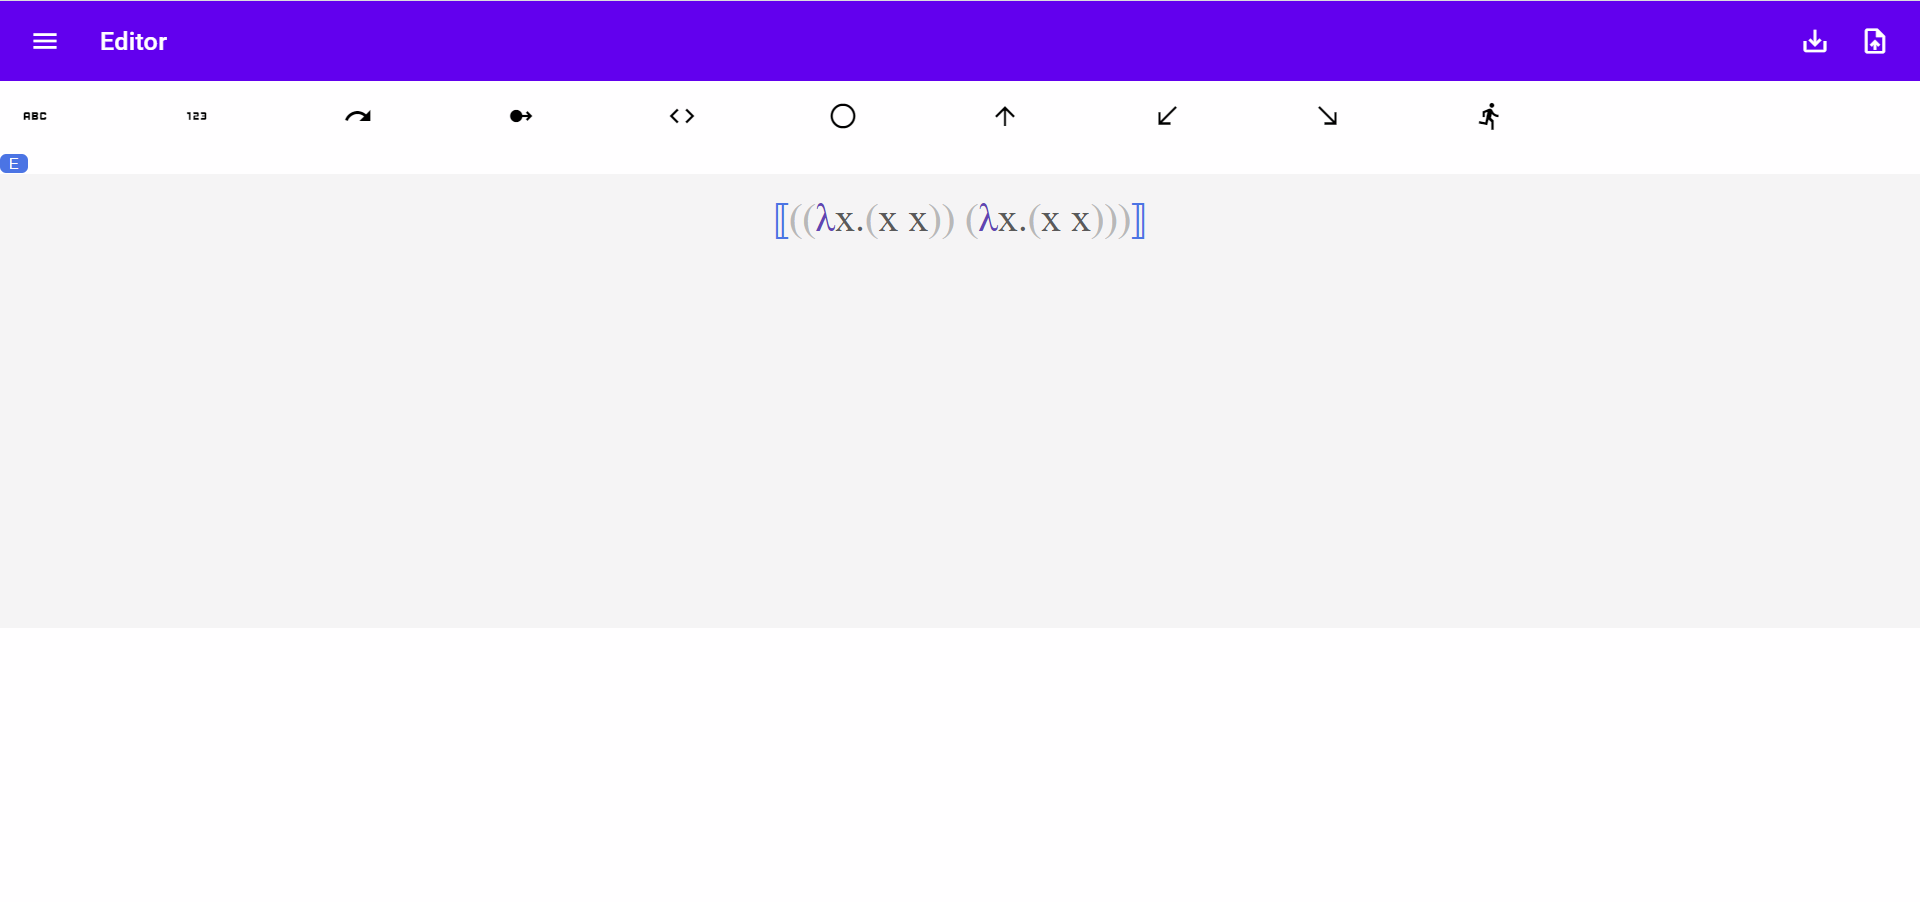
\includegraphics[width=\textwidth]{../assets/editor.png}}
\end{frame}

\subsection{Visualizing ASTs}

\begin{frame}
    \frametitle{User Interface}
    \framesubtitle{Visualizing ASTs}
    \setbeamercovered{transparent}

    \begin{columns}
        \begin{column}{0.5\textwidth}
            \begin{itemize}
                \item Fixed scale
                    \pause
                \item View follows the cursor
                    \pause
                \item Custom zoom level
                    \pause
                \item Folding
                    \pause
                \item Constraints: Cursor jumps
            \end{itemize}
        \end{column}

        \begin{column}{0.5\textwidth}
            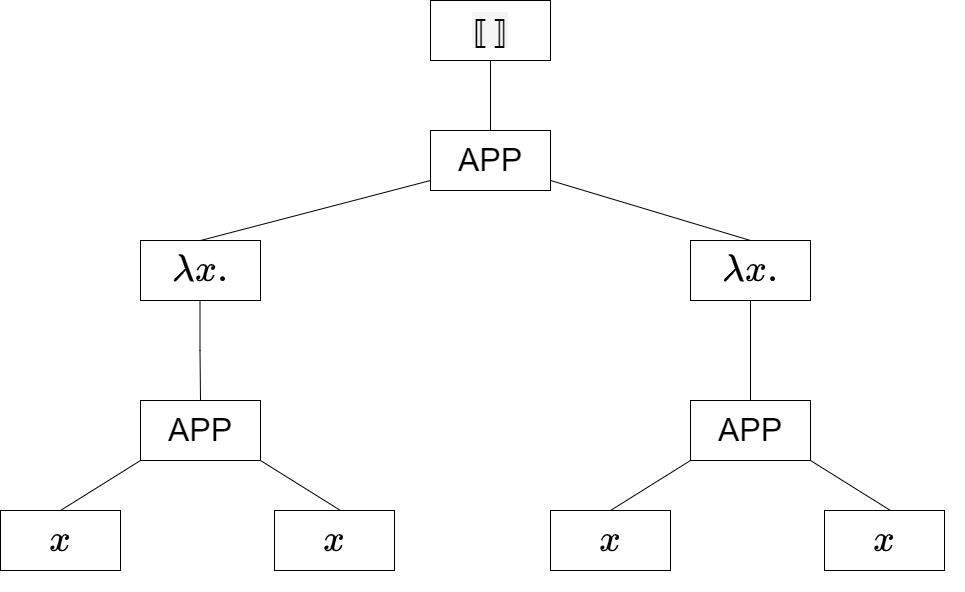
\includegraphics[width=\textwidth]{../assets/ast_root_cursor.png}
            \phantom{Forced spacing}
            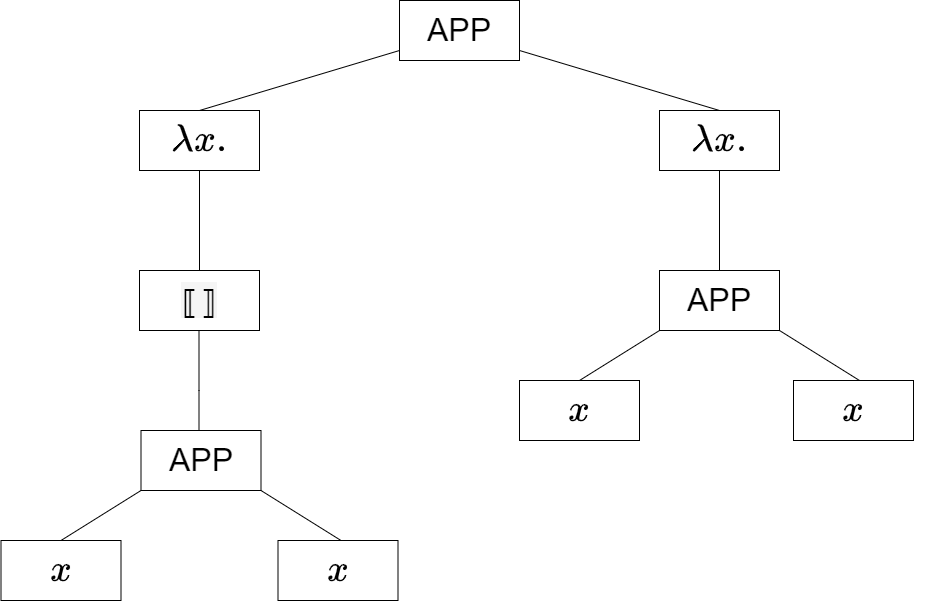
\includegraphics[width=\textwidth]{../assets/ast_subtree_cursor.png}
        \end{column}
    \end{columns}
\end{frame}

\subsection{Editor Expression Builder}

\begin{frame}
    \frametitle{User Interface}
    \framesubtitle{Editor Expression Builder}
    \setbeamercovered{transparent}

    \begin{columns}
        \begin{column}{0.5\textwidth}
            \begin{itemize}
                \item Editor expression holes
                    \pause
                \item Editor expression completeness
                    \pause
                \item Substitute hole with atomic editor expression
                \begin{itemize}
                    \item Click on a hole
                    \item Choose from list
                    \item Repeat until completed
                \end{itemize}
                \pause
                \item Save as macro
            \end{itemize}
        \end{column}

        \begin{column}{0.5\textwidth}
            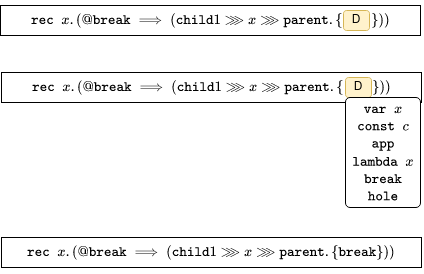
\includegraphics[width=\textwidth]{../assets/exp-builder.png}
        \end{column}
    \end{columns}
\end{frame}

\section{Modelling}

\subsection{ASTs}

\begin{frame}[fragile]
    \frametitle{Modelling}
    \framesubtitle{ASTs}

    \begin{columns}
        \begin{column}{0.5\textwidth}
\begin{lstlisting}[basicstyle=\scriptsize]
type Ast
    = Var Var.Id
    | Con Const.Value
    | App Ast Ast
    | Lambda Var.Id Ast
    | Break Ast
    | Hole

type C
    = Cursor Ast
    | CApp1 C Ast
    | CApp2 Ast C
    | CLambda Var.Id C
    | CBreak C
\end{lstlisting}
            \begin{itemize}
                \item The cursor context is an opaque type
            \end{itemize}
        \end{column}

        \begin{column}{0.5\textwidth}
            \begin{align*}
                \Ast \\\\ \C \\ \aHat \\ \aDot
            \end{align*}
        \end{column}
    \end{columns}
\end{frame}

\subsection{Editor Expressions}

\begin{frame}
    \frametitle{Modelling}
    \framesubtitle{Editor Expressions}

    \begin{definition}
        \begin{align*}
            \Edt \\ \Aep \\ \Aam \\ \Eed
        \end{align*}
    \end{definition}
\end{frame}

\begin{frame}[fragile]
    \frametitle{Modelling}
    \framesubtitle{Editor Expressions}

    \begin{definition}
        \begin{align*}
            \Edt
        \end{align*}
    \end{definition}

\begin{lstlisting}
type Edt
    = Pre Aep Edt
    | Bicond Eed Edt Edt
    | SeqComp Edt Edt
    | Rec Var.Id Edt
    | Call Var.Id
    | Nil
\end{lstlisting}
\end{frame}

\begin{frame}[fragile]
    \frametitle{Modelling}
    \framesubtitle{Unit \& Void}
    \setbeamercovered{transparent}

    \begin{itemize}
        \item Unit
        \begin{itemize}
            \item A type with one constructor which is exposed
            \item Can be constructed at any point from nothing
            \item In elm
\begin{lstlisting}
type ()
    = ()
\end{lstlisting}
        \pause

        \end{itemize}
        \item Void
        \begin{itemize}
            \item A type without any constructors
            \item Can never be constructed
            \item In elm
\begin{lstlisting}
type Never
\end{lstlisting}
        \end{itemize}
    \end{itemize}
\end{frame}

\begin{frame}[fragile]
    \frametitle{Modelling}
    \framesubtitle{Editor Expressions}

\begin{lstlisting}
type Edt
    = Pre Aep Edt
    | Bicond Eed Edt Edt
    | SeqComp Edt Edt
    | Rec Var.Id Edt
    | Call Var.Id
    | Nil

type Aep = ...
type Aam = ...
type Eed = ...
\end{lstlisting}
\end{frame}

\begin{frame}[fragile]
    \frametitle{Modelling}
    \framesubtitle{Editor Expressions}

\begin{lstlisting}
type Edt a
    = Pre (Aep a) (Edt a)
    | Bicond (Eed a) (Edt a) (Edt a)
    | SeqComp (Edt a) (Edt a)
    | Rec Var.Id (Edt a)
    | Call Var.Id
    | Nil
    | EdtHole a

type Aep a = ...
type Aam a = ...
type Eed a = ...
\end{lstlisting}
\end{frame}

\begin{frame}[fragile]
    \frametitle{Modelling}
    \framesubtitle{Editor Expressions}

\begin{lstlisting}
type Edt a
    = Pre (Aep a) (Edt a)
    | Bicond (Eed a) (Edt a) (Edt a)
    | SeqComp (Edt a) (Edt a)
    | Rec Var.Id (Edt a)
    | Call Var.Id
    | Nil
    | EdtHole a

type Aep a = ...
type Aam a = ...
type Eed a = ...


type alias Uncompleted
    = Edt ()

type alias Completed
    = Edt Never
\end{lstlisting}
\end{frame}

\section{Evaluation}

\begin{frame}[fragile]
    \frametitle{Evaluation}
    \framesubtitle{Configurations}
    \setbeamercovered{transparent}

    \begin{itemize}
        \item General signature for evaluation:
\begin{lstlisting}
edt -> WellFormedAst -> WellFormedAst
\end{lstlisting}
            \pause
        \item Use case-of expressions to exhaustively handle all cases.
            \pause
        \item Making impossible states impossible
\begin{lstlisting}
never : Never -> a
\end{lstlisting}
    \end{itemize}
\end{frame}

\section{Upcoming}

\begin{frame}
    \frametitle{Upcoming}
    \setbeamercovered{transparent}

    \begin{itemize}
        \item Evaluation of ASTs
            \pause
        \item Type System
            \pause
        \item Further visualization of ASTs
            \pause
        \item Niceties
        \begin{itemize}
            \item Keybinding
                \pause
            \item Save/load functionality
                \pause
            \item Macros
                \pause
            \item Support short-hand notation for editor expressions
                \pause
            \item Undo/redo
        \end{itemize}
    \end{itemize}
\end{frame}

\begin{frame}
    \centering
    \only<1>{
        \huge{Thanks for coming to our TED Talk.}
    }
    \only<2>{
        \huge{Questions?}
    }
\end{frame}

\end{document}
